%%
%% PhysioFlow -- Software Impacts submission (Original Software Publication)
%% Single-column layout, per the official OSP template. Compiles with a
%% standard LaTeX installation (article class; no special class file needed).
%%

\documentclass[11pt, letterpaper]{article}
\usepackage[utf8]{inputenc}
\usepackage[margin=2cm]{geometry}
\usepackage{titlesec}
\usepackage{amssymb}
\usepackage{graphicx}
\usepackage{booktabs}
\usepackage{makecell}
\usepackage[numbers,sort&compress]{natbib}
\usepackage{tikz}
\usetikzlibrary{positioning, arrows.meta, shapes.geometric}
\usepackage{xurl}
\usepackage{hyperref}
\hypersetup{colorlinks=true, linkcolor=blue, citecolor=blue, urlcolor=blue}
\setlength{\parindent}{0pt}
\setlength{\parskip}{0.5em}

\begin{document}

\begin{center}
{\LARGE\bfseries PhysioFlow: an open-source interactive platform for crop ecophysiology and agronomic data analysis with statistical and experimental-design guard-rails}
\end{center}

\noindent
Daniel Hil\'ario da Silva\textsuperscript{a,*}, Leandro Rodrigues da Silva Souza\textsuperscript{b,c}, Andr\'e Abade\textsuperscript{d}, Francisco de Almeida Lobo\textsuperscript{e}, Fernando Rodrigues Cabral Filho\textsuperscript{b,c}, Erli Pinto dos Santos\textsuperscript{f}, Adinan Alves da Silva\textsuperscript{c}, Daiane Alves da Silva\textsuperscript{b}, Ketlyn Santos Sousa\textsuperscript{c}, Igor Eli da Silva\textsuperscript{c}, Alan Carlos da Costa\textsuperscript{c}

\vspace{0.4em}
\noindent
{\footnotesize
\textsuperscript{a}Instituto Federal Goiano, Campus Catal\~ao, Goi\'as, Brazil\\
\textsuperscript{b}Centro de Excel\^encia em Agricultura Exponencial (CEAGRE), Rio Verde, Goi\'as, Brazil\\
\textsuperscript{c}Instituto Federal Goiano, Campus Rio Verde, Goi\'as, Brazil\\
\textsuperscript{d}Instituto Federal de Mato Grosso, Cuiab\'a, Mato Grosso, Brazil\\
\textsuperscript{e}Universidade Federal de Mato Grosso, Mato Grosso, Brazil\\
\textsuperscript{f}Universidade Federal Rural do Rio de Janeiro, Serop\'edica, Rio de Janeiro, Brazil\\[0.3em]
\textsuperscript{*}Corresponding author: \texttt{daniel.hilario@ifgoiano.edu.br}\\[0.3em]
ORCID: Daniel Hil\'ario da Silva: 0000-0002-0800-065X; Leandro Rodrigues da Silva Souza: 0000-0003-2477-6893; Andr\'e Abade: 0000-0001-9771-9123; Francisco de Almeida Lobo: 0000-0002-5670-0351; Fernando Rodrigues Cabral Filho: 0000-0002-5090-5946; Erli Pinto dos Santos: 0000-0002-4888-906X; Adinan Alves da Silva: 0000-0002-1589-6773; Daiane Alves da Silva: 0009-0004-8550-6576; Ketlyn Santos Sousa: 0009-0001-5682-3925; Igor Eli da Silva: 0000-0001-8897-152X; Alan Carlos da Costa: 0000-0001-9339-9257.
}

\begin{abstract}
\emph{PhysioFlow} is an open-source Python/Streamlit platform for crop-ecophysiology and general agronomic or biological data. It ingests CSV/TSV/XLSX exports, validates them against an explicit schema, and offers a configurable replicate pipeline, exploratory analysis with statistical guard-rails (confounding, multicollinearity, normality and multi-method outlier checks), supervised regression and classification with optional GroupKFold, geospatial analysis in UTM metres, STL decomposition, and a formal experimental-design module (from completely randomised and block designs to factorial, Latin square, split-plot, strip-plot, nested, ANCOVA and dose-response) cross-validated against R. An automatic data-profile makes it dataset-agnostic beyond ecophysiology. Released under GPL-2.0, it runs code-free in a trilingual (PT/EN/ES) interface.
\end{abstract}

\vspace{0.5em}
\noindent\textbf{Keywords:} Crop ecophysiology; IRGA; Exploratory data analysis; Experimental design; Statistical guard-rails; Reproducible research
\vspace{0.5em}

%% ====================================================================
\section*{Code metadata}

\begin{table}[htbp]
\centering
\footnotesize
\begin{tabular}{|l|p{4.7cm}|p{6.3cm}|}
\hline
\textbf{Nr.} & \textbf{Code metadata description} & \textbf{Value} \\
\hline
C1 & Current code version & v1.0 \\
\hline
C2 & Permanent link to code/repository used for this code version & \url{https://github.com/ML-Carbon-Project/physioFlow} \\
\hline
C3 & Permanent link to reproducible capsule & \url{https://github.com/ML-Carbon-Project/physioFlow} \\
\hline
C4 & Legal code license & GPLv2 with mandatory citation clause \\
\hline
C5 & Code versioning system used & git \\
\hline
C6 & Software code languages, tools and services used & Python 3.10+; Streamlit; pandas, NumPy, SciPy, scikit-learn, statsmodels; geopandas, shapely, pyproj, libpysal, esda; pytest \\
\hline
C7 & Compilation requirements, operating environments \& dependencies & Linux, macOS, Windows; Python $\geq 3.10$; \texttt{pip install -r requirements.txt} \\
\hline
C8 & If available, link to developer documentation/manual & \url{https://github.com/ML-Carbon-Project/physioFlow/tree/main/docs} \\
\hline
C9 & Support email for questions & \texttt{daniel.hilario@ifgoiano.edu.br} \\
\hline
\end{tabular}
\caption{Code metadata.}
\label{tbl:metadata}
\end{table}

%% ====================================================================
\section{Introduction}\label{sec:intro}

Plant ecophysiology links the carbon, water and energy economy of crops to their environment, and its field measurement underpins decisions in agronomy, breeding and climate-change adaptation~\cite{Lambers2008,Long2006}. Three portable instruments dominate field campaigns: infrared gas analyzers (IRGA) measure net photosynthesis ($A$), transpiration ($E$), stomatal conductance ($g_s$) and internal/ambient CO$_2$, from which derived efficiencies such as WUE, $A/C_i$ and $C_i/C_a$ are computed~\cite{Farquhar1980,vonCaemmerer2000,Long2003}; chlorophyll fluorometers and content meters report $Y_{II}$, the electron transport rate and chlorophyll $a$/$b$~\cite{Maxwell2000,Baker2008}; and ceptometers estimate the leaf area index~\cite{Breda2003}. Together they characterise crop photosynthetic performance across genotypes, phenological stages and seasons, anchoring studies of responses to irrigation, salinity and soil management~\cite{Oliveira2017,Munjonji2021,Peters2012,Sanchez2003,Guarrera2024}, central in the Brazilian Cerrado to both yield and ecosystem carbon accounting~\cite{Vourlitis2022}.

Each instrument exports a wide CSV/XLSX table whose rows are leaf or canopy measurements with gas-exchange, fluorescence, chlorophyll and LAI variables plus metadata (crop, farm, land use, season, coordinates, date). Turning this raw output into a publishable analysis still demands several non-trivial steps: standardising categorical fields, discarding rows without minimum metadata, consolidating chlorophyll and LAI replicates, running exploratory and inferential analyses, checking multicollinearity among derived indices, inspecting spatial structure, decomposing temporal trends and, optionally, fitting predictive models.

Despite the wide availability of these instruments, manufacturers provide no free, open-source software for the exploratory and modelling stages that turn raw exports into results; vendor viewers focus on acquisition and quality control. Researchers must therefore write custom scripts in R~\cite{Rcore} or Python, a considerable barrier for those without programming or statistics training. In most laboratories these steps are still done by hand or half-automated across spreadsheets and disconnected packages, which is slow, error-prone, hard to reproduce, and, in high-throughput campaigns, the bottleneck of the whole analysis. The structure of ecophysiology field data also invites silent statistical errors: physiological indices are mutually derived (e.g.\ WUE $= A/E$), inflating multicollinearity by construction; sampling designs frequently alias farm, crop and land use, so an apparent ``between-farm'' difference may be an unidentifiable ``between-crop'' difference; replicated measurements at the same site induce pseudoreplication~\cite{Hurlbert1984} that inflates model skill; and short campaigns offer too few dates for meaningful seasonal decomposition.

Inspired by recent open-source efforts that bridged data analysis and end users via Streamlit~\cite{Streamlit,daSilva2025Parkinson,DaSilva2026Goias}, we developed \emph{PhysioFlow} to consolidate the entire ecophysiology data-analysis workflow into a single configurable, interactive platform. The distinguishing design choice is a set of \emph{statistical guard-rails} woven into the user interface: the application not only computes statistics but warns when their assumptions are violated. Recent software papers in neighbouring agronomic niches~\cite{Magala2026apsimNGpy,Crecco2026prismatools} have shown how much is gained by releasing an instrument-bound, end-to-end analytical pipeline as citable software, and PhysioFlow does the same for crop ecophysiology.

%% ====================================================================
\section{Software description}\label{sec:software}

\subsection{Software architecture}\label{sec:arch}

\emph{PhysioFlow} is implemented in Python~3.10~\cite{Streamlit,McKinney2010,Harris2020} and follows a session-state, page-renderer pattern in which each of nine user-facing pages reads from a shared \texttt{st.session\_state} and consumes the cleaning, statistics and visualisation primitives in \texttt{src/}, so costly I/O and cleaning happen at most once per session (Fig.~\ref{fig:architecture}). A resolver (\texttt{src/profile.py}) matches the uploaded frame against the reference schema and selects the \emph{data-profile}: the physiology profile (domain defaults, presets and schema report) when the columns match, otherwise a generic profile that drops those presets so any agronomic or biological table is analysed without code changes.

\begin{figure}[htbp]
\centering
\resizebox{\linewidth}{!}{%
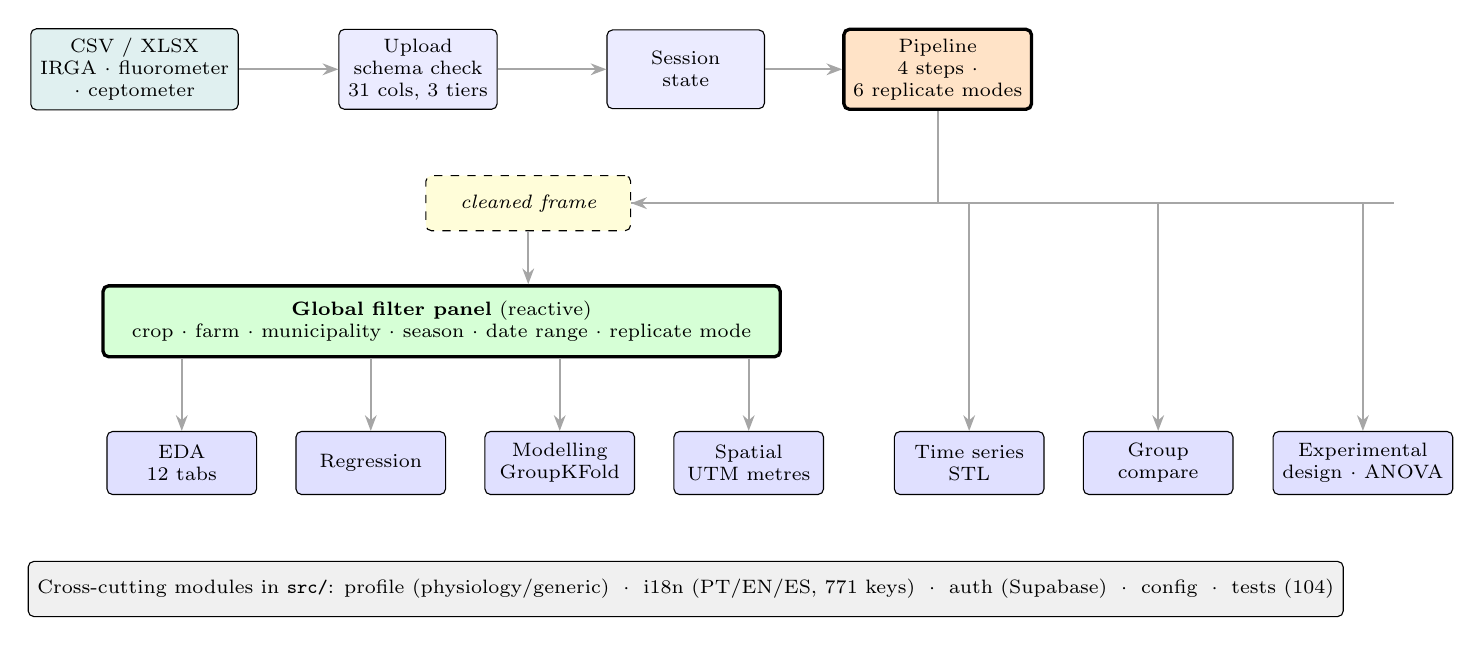
\begin{tikzpicture}[
  font=\scriptsize,
  src/.style={draw, rounded corners=2pt, minimum width=21mm, minimum height=10mm, fill=teal!12, align=center},
  proc/.style={draw, rounded corners=2pt, minimum width=20mm, minimum height=10mm, fill=blue!8, align=center},
  gate/.style={draw, rounded corners=2pt, minimum width=23mm, minimum height=10mm, fill=orange!22, align=center, very thick},
  frame/.style={draw, dashed, rounded corners=2pt, minimum width=26mm, minimum height=7mm, fill=yellow!15, align=center, font=\scriptsize\itshape},
  filt/.style={draw, rounded corners=2pt, minimum height=9mm, fill=green!16, align=center, very thick},
  page/.style={draw, rounded corners=2pt, minimum width=19mm, minimum height=8mm, fill=blue!12, align=center},
  band/.style={draw, rounded corners=2pt, minimum width=152mm, minimum height=7mm, fill=gray!12, align=center},
  arr/.style={->, >=Stealth, semithick, gray!70}
]
% --- ingestion row ---
\node[src]  (csv)      at (0,0)   {CSV / XLSX\\\scriptsize IRGA $\cdot$ fluorometer\\\scriptsize $\cdot$ ceptometer};
\node[proc] (upload)   at (3.6,0) {Upload\\\scriptsize schema check\\\scriptsize 31 cols, 3 tiers};
\node[proc] (state)    at (7.0,0) {Session\\state};
\node[gate] (pipeline) at (10.2,0){Pipeline\\\scriptsize 4 steps $\cdot$\\\scriptsize 6 replicate modes};
\draw[arr] (csv) -- (upload);
\draw[arr] (upload) -- (state);
\draw[arr] (state) -- (pipeline);

% --- cleaned frame ---
\node[frame] (cf) at (5.0,-1.7) {cleaned frame};
\draw[arr] (pipeline.south) |- (cf.east);

% --- global reactive filter (over the four analytical pages) ---
\node[filt, minimum width=86mm] (filter) at (3.9,-3.2)
  {\textbf{Global filter panel} (reactive)\\\scriptsize crop $\cdot$ farm $\cdot$ municipality $\cdot$ season $\cdot$ date range $\cdot$ replicate mode};
\draw[arr] (cf.south) -- (cf.south|-filter.north);

% --- analytical pages ---
\node[page] (eda)     at (0.6,-5.0) {EDA\\\scriptsize 12 tabs};
\node[page] (reg)     at (3.0,-5.0) {Regression};
\node[page] (model)   at (5.4,-5.0) {Modelling\\\scriptsize GroupKFold};
\node[page] (spatial) at (7.8,-5.0) {Spatial\\\scriptsize UTM metres};
\node[page] (ts)      at (10.6,-5.0){Time series\\\scriptsize STL};
\node[page] (cmp)     at (13.0,-5.0){Group\\compare};
\node[page] (exp)     at (15.6,-5.0){Experimental\\\scriptsize design $\cdot$ ANOVA};

\draw[arr] (eda.north|-filter.south)     -- (eda.north);
\draw[arr] (reg.north|-filter.south)     -- (reg.north);
\draw[arr] (model.north|-filter.south)   -- (model.north);
\draw[arr] (spatial.north|-filter.south) -- (spatial.north);
% time series, group comparison and experimental design read the cleaned frame directly
\draw[semithick, gray!70] (cf.east) -- (16.0,-1.7);
\draw[arr] (10.6,-1.7) -- (ts.north);
\draw[arr] (13.0,-1.7) -- (cmp.north);
\draw[arr] (15.6,-1.7) -- (exp.north);

% --- cross-cutting band ---
\node[band] (cross) at (7.0,-6.6)
  {Cross-cutting modules in \texttt{src/}: profile (physiology/generic) \;$\cdot$\; i18n (PT/EN/ES, 771 keys) \;$\cdot$\; auth (Supabase) \;$\cdot$\; config \;$\cdot$\; tests (104)};
\end{tikzpicture}%
}
\caption{High-level data-flow architecture of \emph{PhysioFlow}. Raw exports from IRGA, chlorophyll fluorometer, and ceptometer instruments are validated against the reference schema upon upload, cached in the Streamlit session state, and consumed by the Pipeline, which produces a single cleaned frame. A shared, reactive \emph{global filter panel} (crop, farm, municipality, season, date range, and replicate mode) is injected at the top of the four analytical pages (EDA, Regression, Modelling, Spatial) and propagates instantly to every chart, test and model; the Time Series, Group-comparison and Experimental-design pages read the cleaned frame directly through their own controls. Library stack: Pipeline $\to$ \texttt{pandas}/\texttt{NumPy}; modelling $\to$ \texttt{scikit-learn}~\cite{Pedregosa2011}; inference $\to$ \texttt{SciPy}/\texttt{statsmodels}; visualisation $\to$ \texttt{seaborn}~\cite{Waskom2021,Hunter2007}; geospatial $\to$ \texttt{geopandas}, \texttt{pyproj}, \texttt{libpysal}/\texttt{esda}~\cite{Rey2007Pysal}.}\label{fig:architecture}
\end{figure}

The \texttt{src/} package is organised by concern: \texttt{schema.py} validates 31 reference columns in three severity tiers without blocking the upload; \texttt{pipeline.py} holds the deterministic cleaning primitives; \texttt{stats\_utils.py} implements bias-corrected Cram\'er's V~\cite{Bergsma2013}, the confounding auditor and the analysis-of-variance routines behind the experimental-design page (split-plot, strip-plot, nested and ANCOVA models; Scott--Knott, Duncan, LSD, Scheff\'e and Dunnett comparisons), each checked against R; and \texttt{ml/model\_registry.py} declares two \texttt{scikit-learn} pipelines of five regressors~\cite{Breiman2001,Friedman2001} and seven classifiers. Cross-cutting \texttt{i18n/} (771 keys at full PT/EN/ES parity), \texttt{auth/}, \texttt{config/} and \texttt{tests/} (104 \texttt{pytest} functions) serve every page. Public functions carry type annotations, and \texttt{ruff}, \texttt{mypy} and the \texttt{pytest} suite run on Python~3.10--3.12 through a GitHub Actions workflow; new estimators, cleaning primitives and schema columns are registered declaratively.

\subsection{Software functionalities}\label{sec:functions}

\paragraph{Upload (Fig.~\ref{fig:upload}).} Accepts CSV, TSV, TXT (configurable delimiter), XLSX and XLS files. The schema validator classifies every expected column as \emph{required}, \emph{recommended} or \emph{optional}, checks types, flags columns that exist but are 100\% empty, and verifies that latitude/longitude lie within plausible ranges. Missing columns disable dependent features without blocking the upload.

\begin{figure}[htbp]
  \centering
  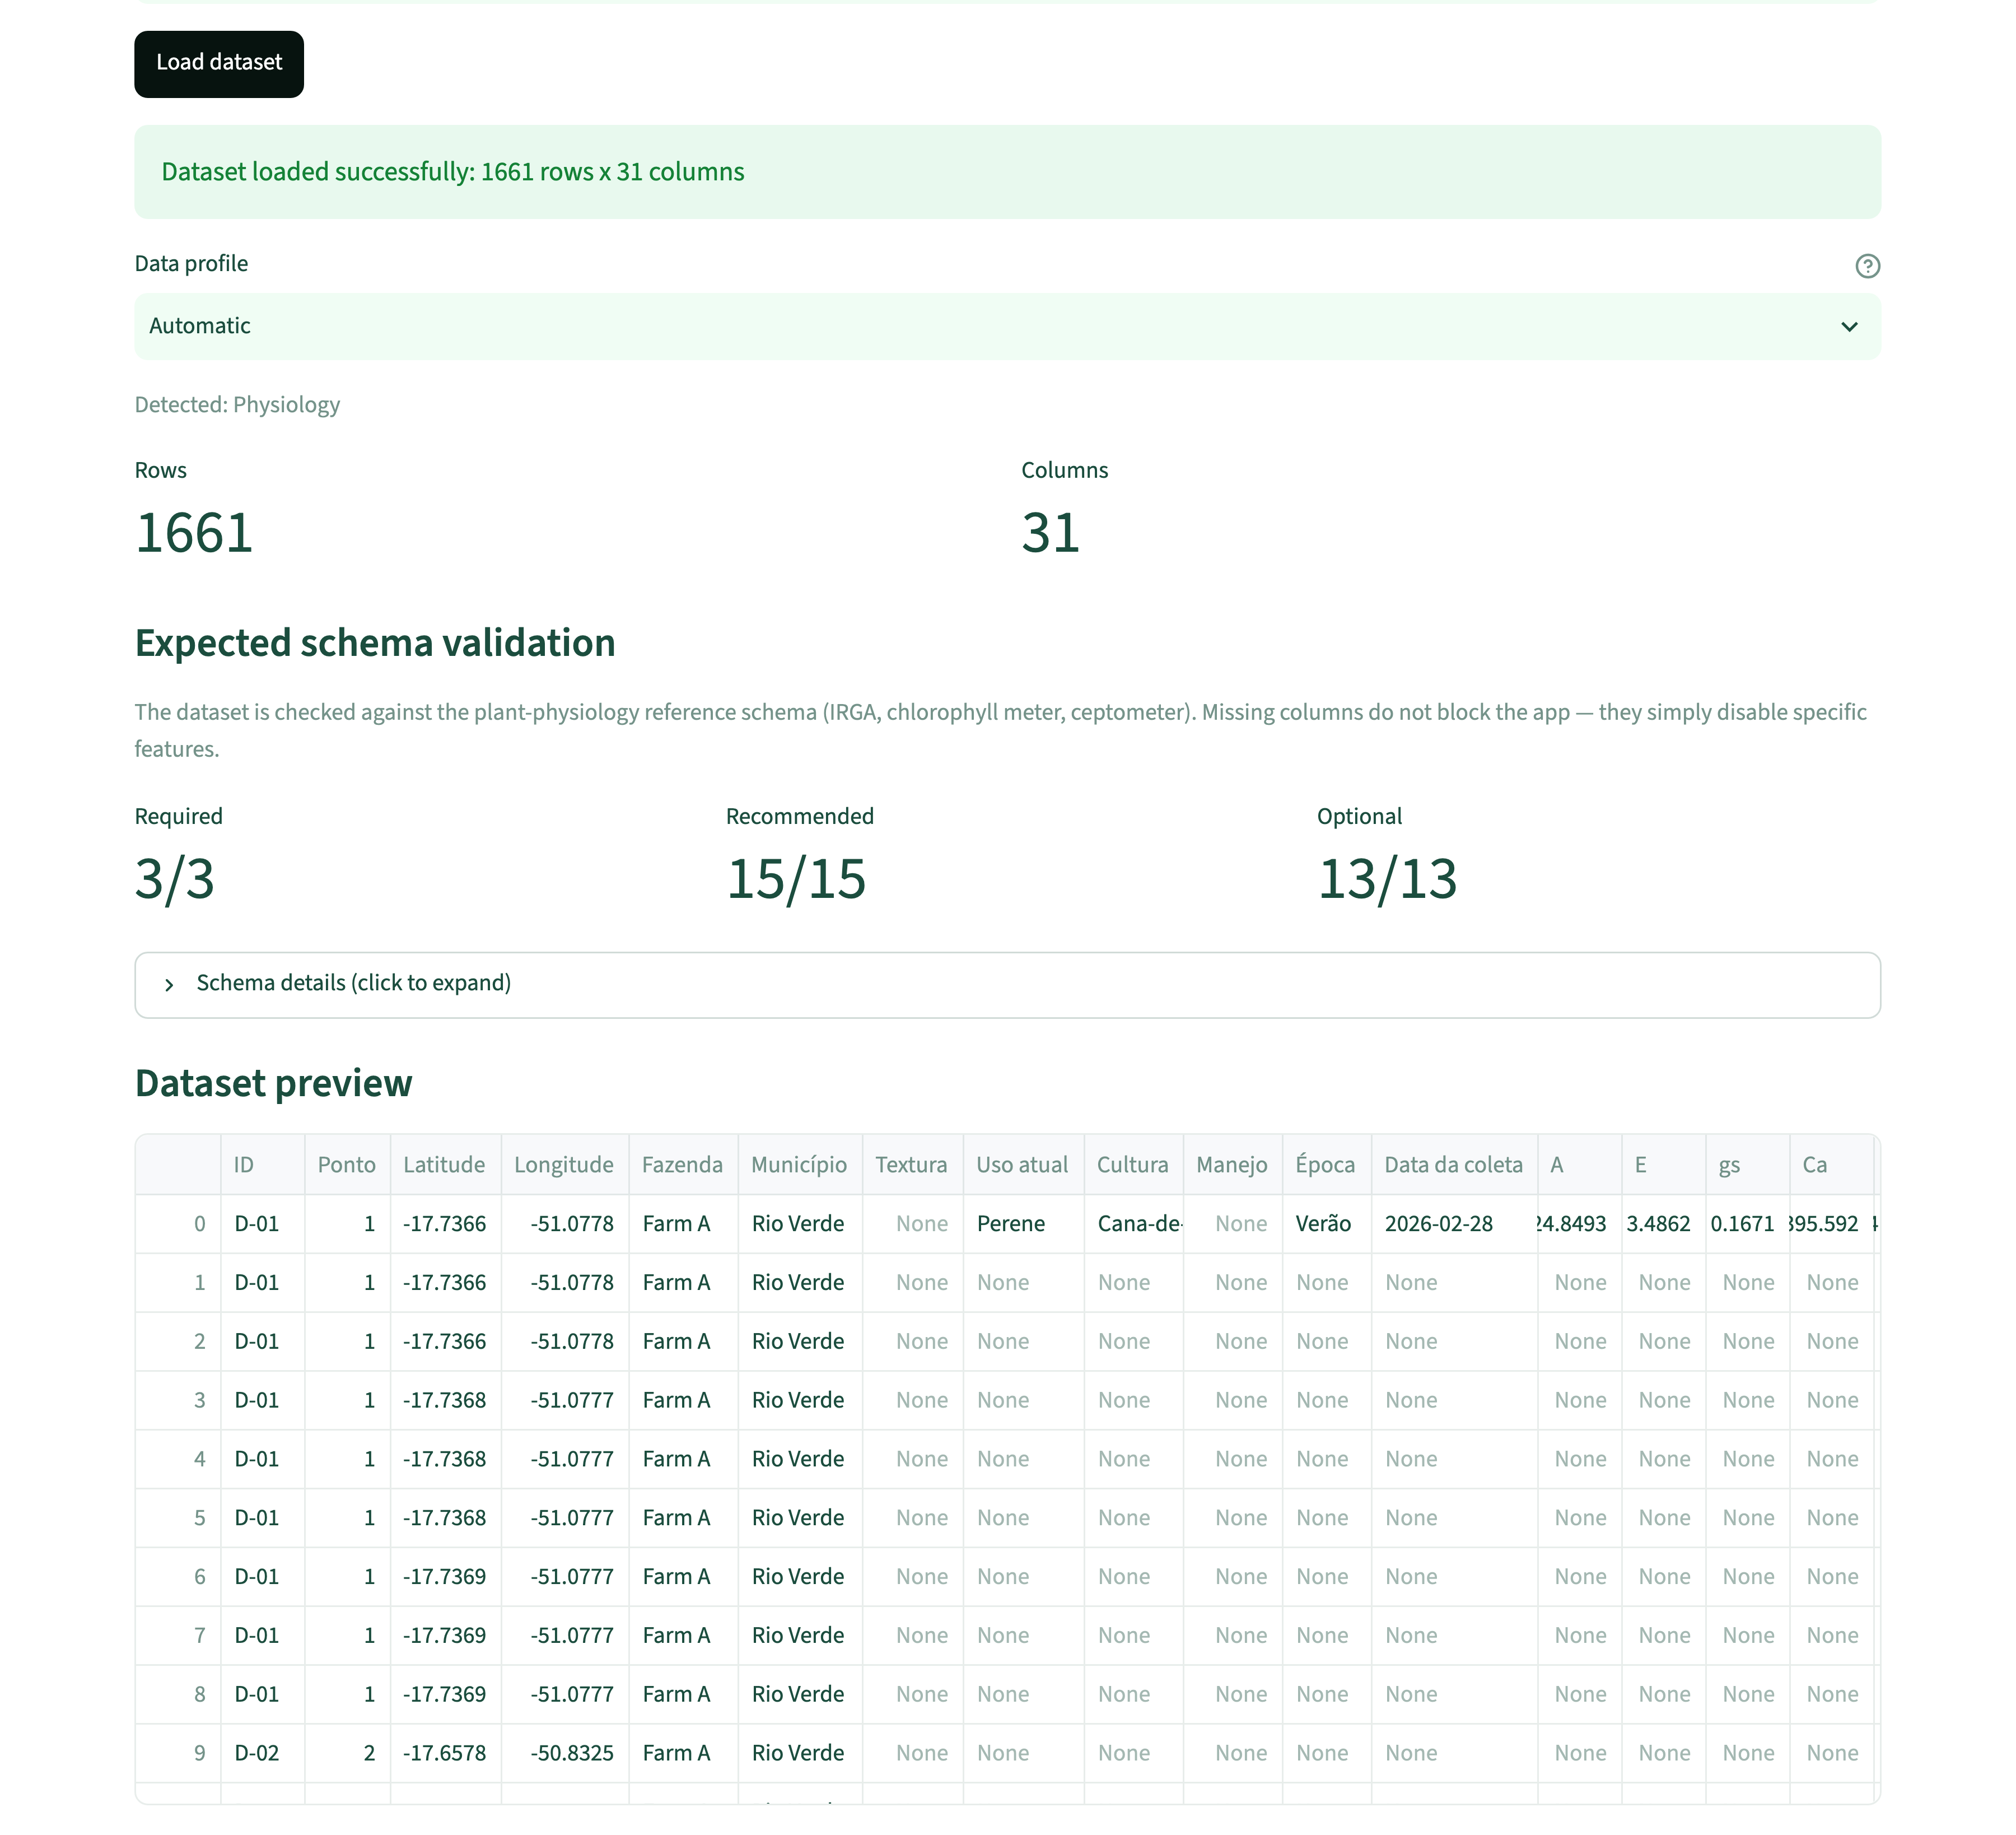
\includegraphics[width=\linewidth]{figs/upload_schema.png}
  \caption{Upload page after ingestion of an ecophysiology dataset. The schema validator reports each expected column with its severity tier, the resolved column name, the detected type and the dependent feature.}\label{fig:upload}
\end{figure}

\paragraph{Pipeline.} Four deterministic steps (text standardisation, removal of rows without essential metadata, removal of empty grid points and replicate treatment) are followed by a step-by-step report (Fig.~\ref{fig:pipeline}) recording rows in/out per step, with a warning whenever a step discards more than 50\% of the rows. Chlorophyll and LAI replicates are handled in six modes: mean, median, replicate-unfolding into independent rows, and exclusive selection of replicate~1, 2 or~3.

\begin{figure}[htbp]
  \centering
  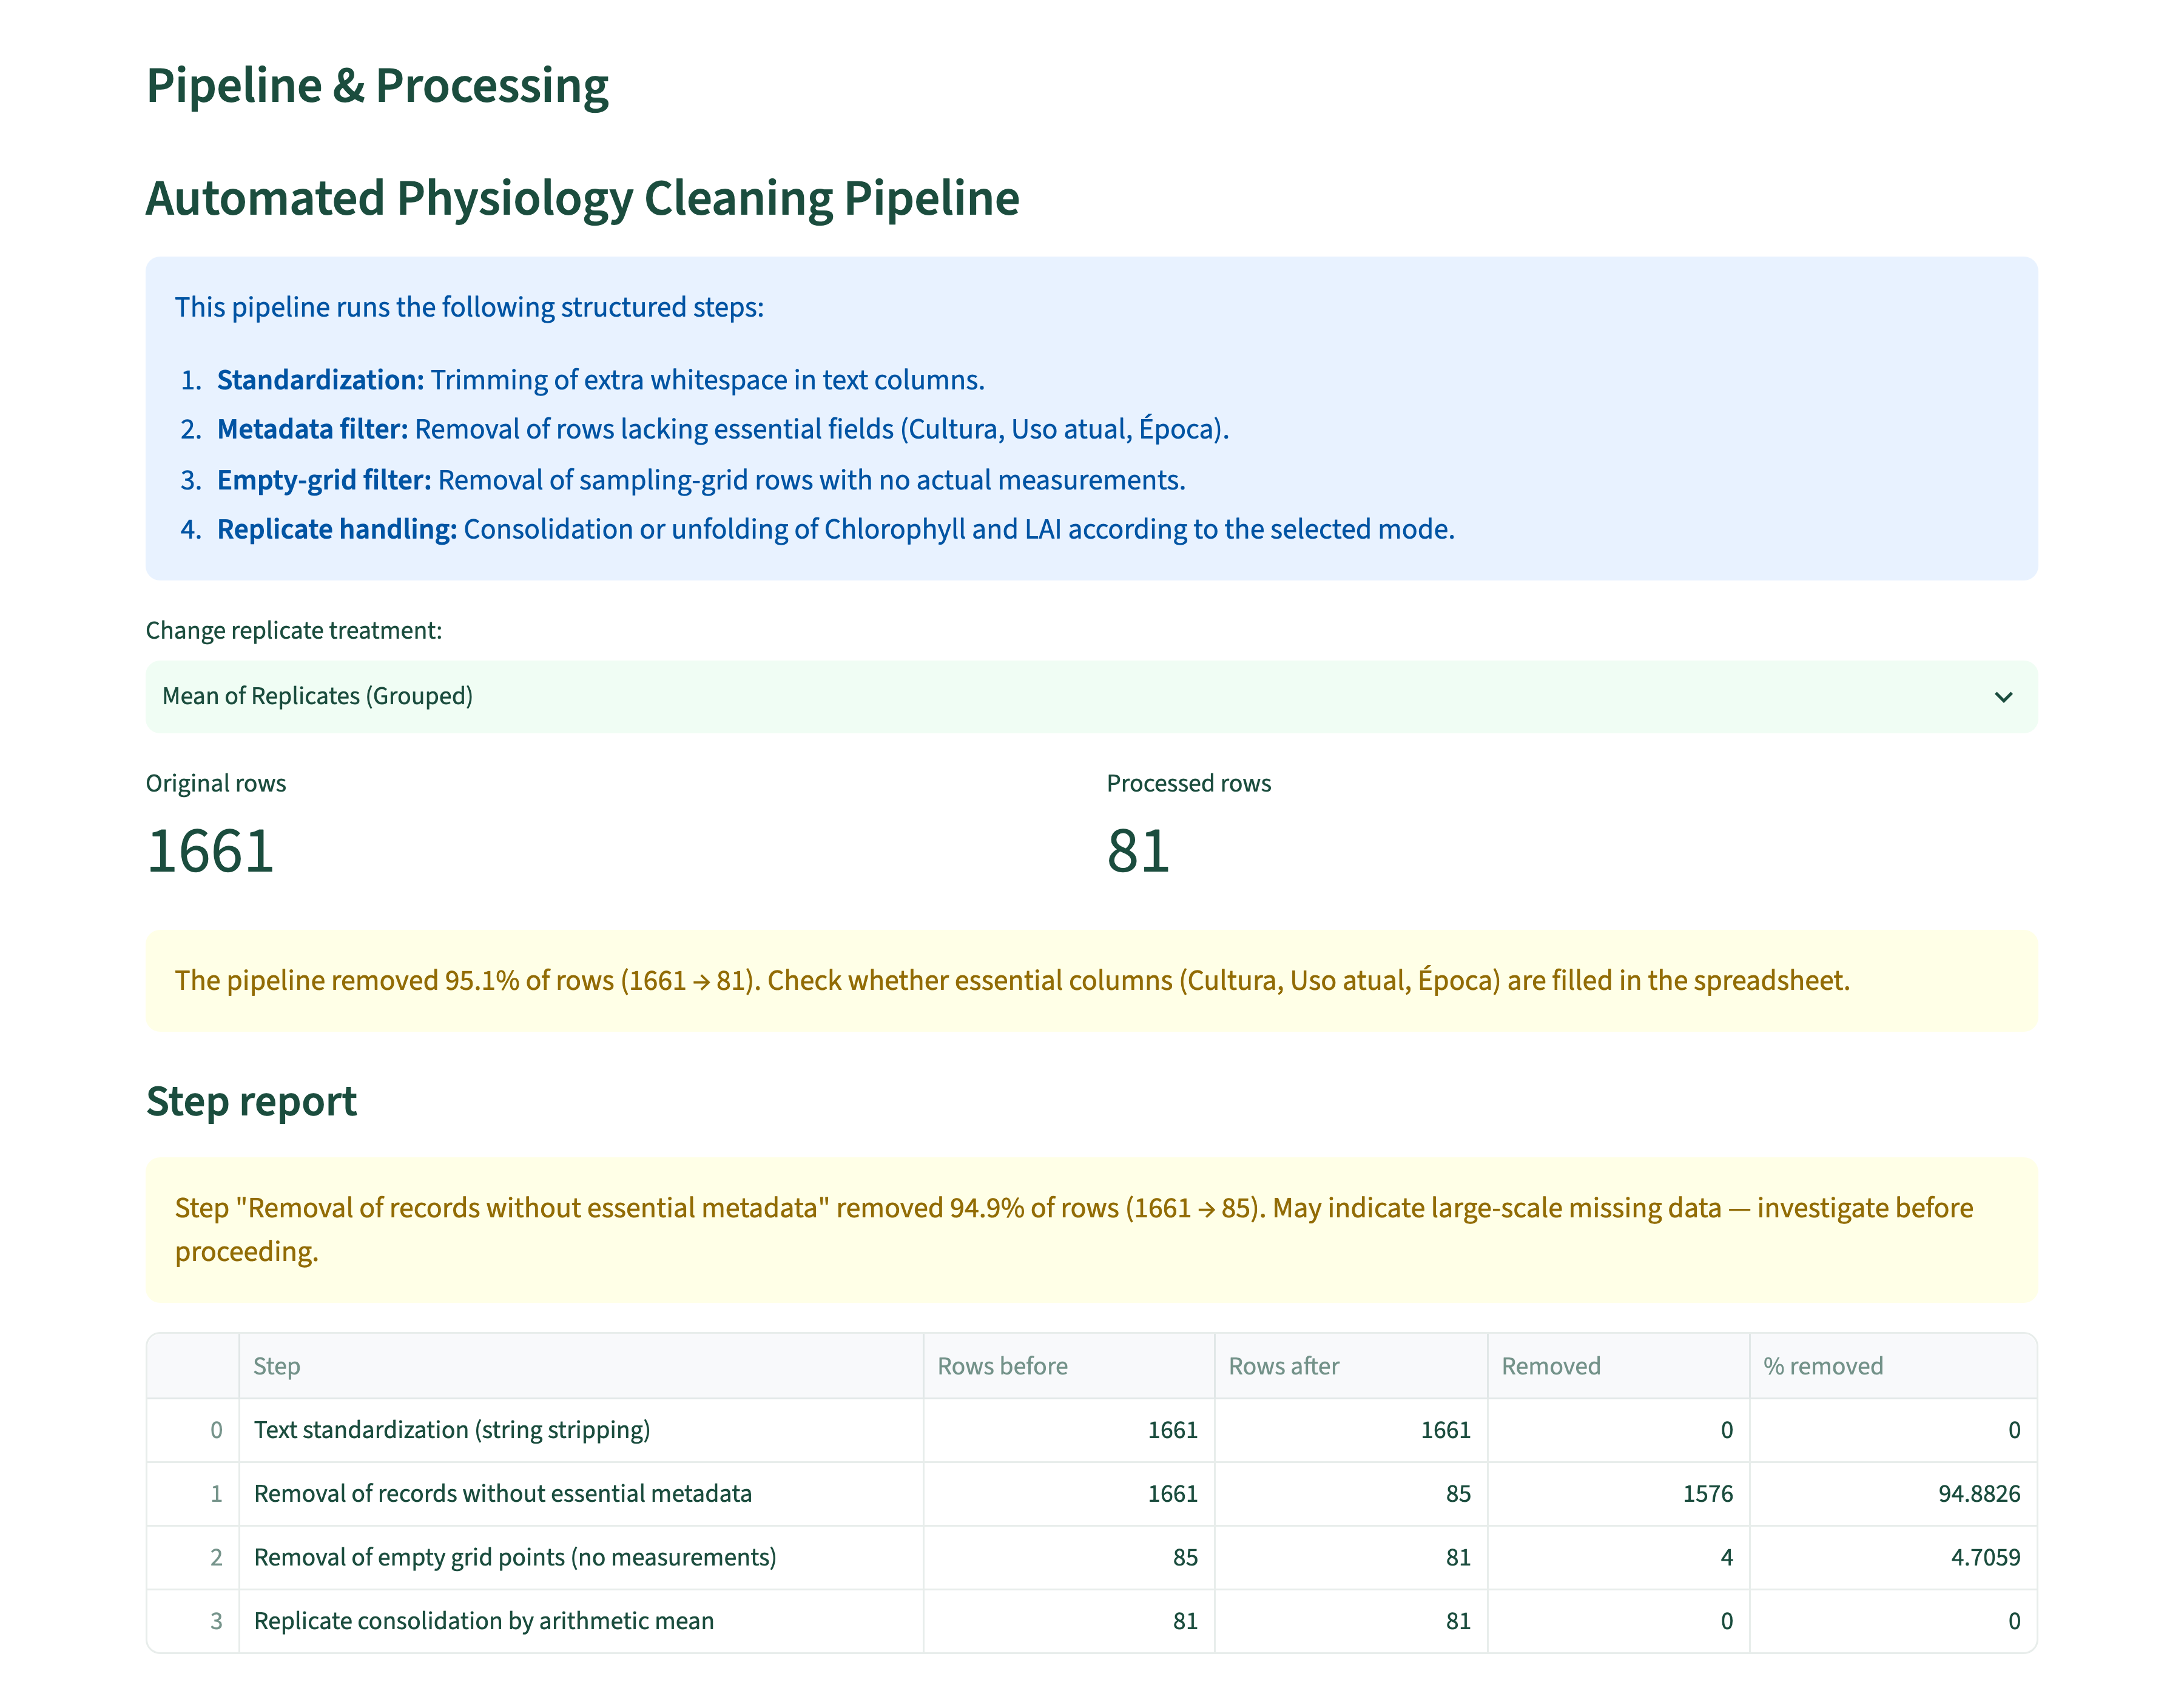
\includegraphics[width=\linewidth]{figs/pipeline_audit.png}
  \caption{Step-by-step audit of the cleaning pipeline applied to the real Rio Verde dataset. Each row reports lines before/after and the share removed; the essential-metadata filter alone removes 94.9\% of the raw rows, triggering the high-discard warning.}\label{fig:pipeline}
\end{figure}

\paragraph{Exploratory Data Analysis.} Twelve tabs cover descriptive statistics; a data-quality tab auditing categorical \emph{confounding} via Cram\'er's V (Fig.~\ref{fig:confounding}); distributions, boxplots, pair plots and Pearson/Spearman/Kendall correlations; a lat/lon map; temporal aggregation and composition charts; non-parametric inference (Kruskal--Wallis~\cite{Kruskal1952} with a minimum-N slider, Shapiro--Wilk~\cite{ShapiroWilk1965} with Q--Q plots, and VIF~\cite{Belsley1980VIF} caveating that derived indices such as $C_i/C_a$, $A/C_i$ and WUE inflate VIF by construction); a top-$N$ hotspots ranking; and a multi-method outlier audit (Z-score, IQR, Isolation Forest~\cite{Liu2008}, Local Outlier Factor~\cite{Breunig2000}, Elliptic Envelope) with a consensus criterion.

\begin{figure}[htbp]
  \centering
  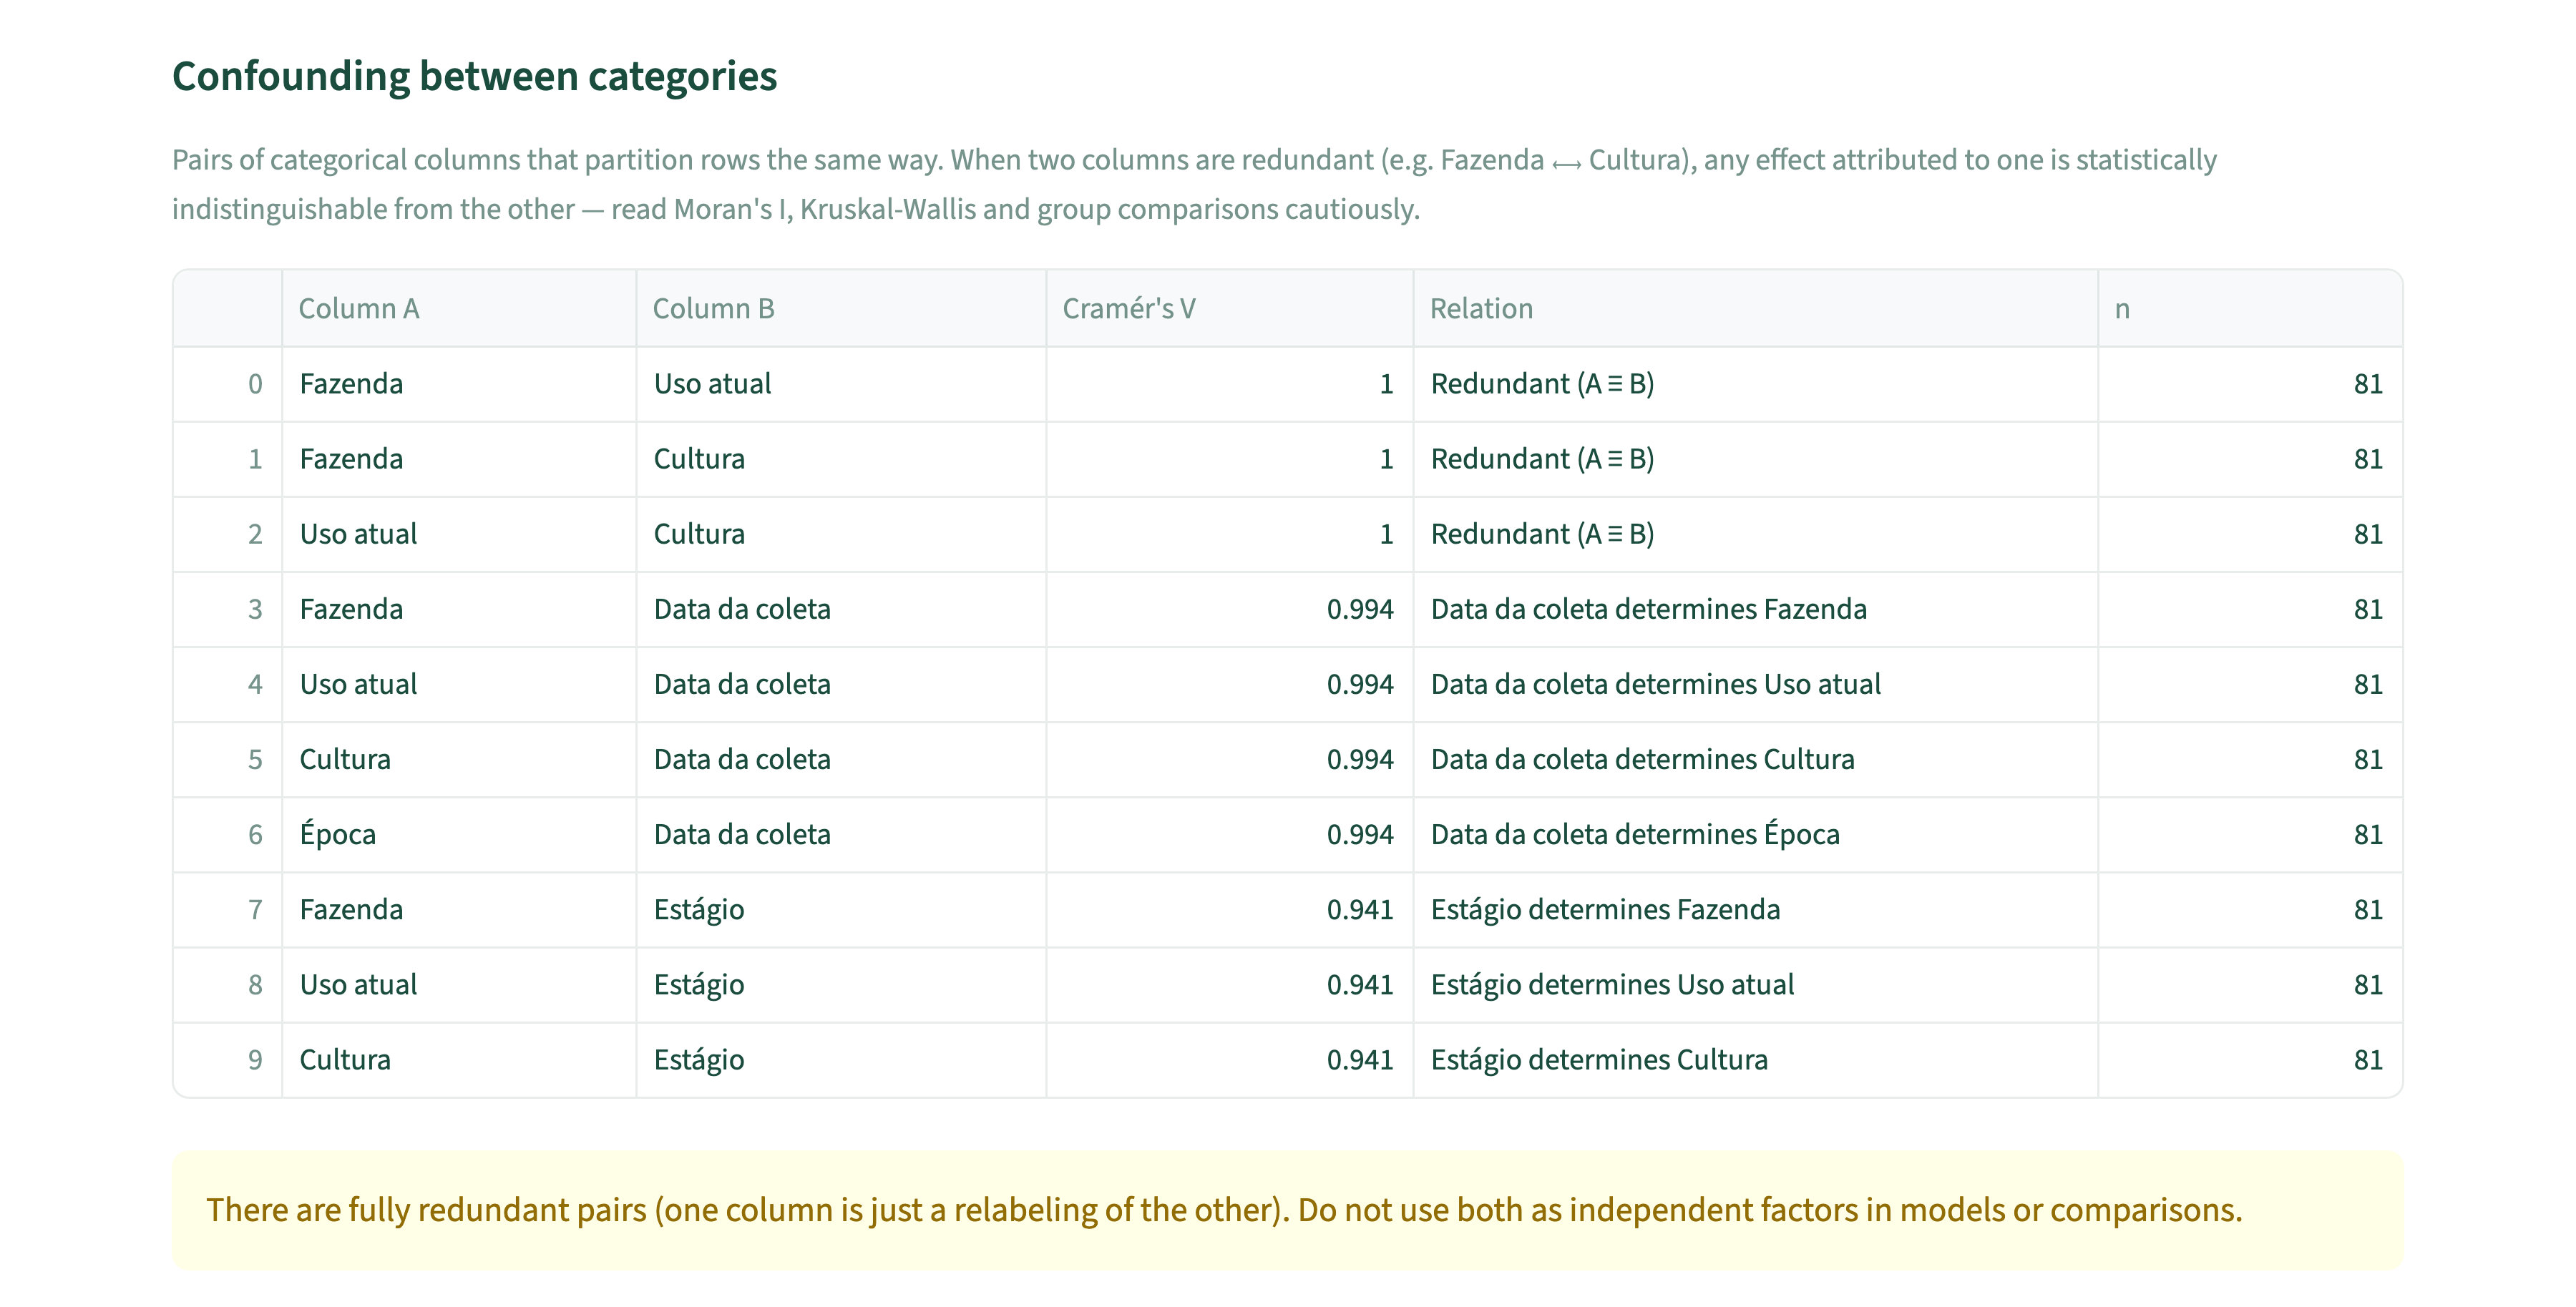
\includegraphics[width=\linewidth]{figs/confounding.png}
  \caption{Data-quality tab auditing categorical confounding. On the Rio Verde dataset the tool detects that \emph{Fazenda} (farm), \emph{Cultura} (crop) and \emph{Uso atual} (land use) are perfectly redundant (Cram\'er's V $=1.00$), warning the user that between-group contrasts on these fields are statistically unidentifiable.}\label{fig:confounding}
\end{figure}

\paragraph{Regression and Modelling.} The Regression page offers physiological bivariate presets (e.g.\ $g_s$ vs.\ $A$) and free custom regression. On the Modelling page the user chooses the task: regression compares five estimators and reports holdout $R^2$, MAE, RMSE and cross-validated $R^2$; classification compares seven and reports accuracy, precision, recall, $F_1$ and a confusion matrix. In both, an \emph{optional GroupKFold} with a grouping-column selector (by default a synthetic \emph{farm + point} key) curbs pseudoreplication~\cite{Hurlbert1984}.

\paragraph{Experimental Design.} A separate page treats the uploaded table as a designed experiment: the user names a categorical treatment factor and a numeric response and chooses the layout, from completely randomised (CRD) and randomised complete block (RCBD) through two- and three-factor factorials to the Latin square and the compound-error split-plot, strip-plot and nested designs; analysis of covariance (ANCOVA) and dose-response regression are also available. The page fits the model, prints the ANOVA table, checks residual normality and homoscedasticity (Shapiro--Wilk, Levene) on screen, and warns on violated assumptions or under-replicated groups. Mean comparison offers Tukey HSD, Scott--Knott~\cite{ScottKnott1974}, Duncan, LSD/Fisher, Scheff\'e and Dunnett as compact-letter displays, with a reproducible code snippet per result; every procedure was validated against its reference R implementation.

\paragraph{Spatial Analysis.} IDW interpolation, global Moran's I and LISA cluster maps~\cite{Anselin1995}, Getis--Ord $G_i^*$~\cite{Getis1992}, UTM grid aggregation and ordinary kriging~\cite{Cressie1993} with a fitted spherical variogram. All distance-based computations run in \emph{UTM metres}, with an EPSG code derived from the mean longitude to correct the anisotropy of degree-based distances.

\paragraph{Time Series.} Daily resampling (mean or median) and STL decomposition~\cite{Cleveland1990STL}, \emph{blocked when fewer than ten distinct dates are present} so that sparse campaigns do not yield a decomposition dominated by interpolation.

\paragraph{Two-group comparison and Authentication.} A comparative page splits the dataset by multi-select or substring pattern and returns a per-variable Mann--Whitney U test~\cite{Mann1947}, paired log-linear regressions and an hourly profile. An optional Supabase login (off by default) adds authentication.

%% ====================================================================
\section{Results and discussion}\label{sec:examples}

\subsection{A crop-ecophysiology campaign}\label{sec:ex-physio}

A de-identified Cerrado campaign from Rio Verde, GO, with 1\,661 raw measurement rows across soybean and sugarcane, was ingested via the Upload page. The schema validator confirmed the required metadata and physiological variables and flagged \emph{Manejo} (soil management) and \emph{Textura} (soil texture) as present but 100\% empty.

The Pipeline was run in the default mean-replicate mode. Its audit trail (Fig.~\ref{fig:pipeline}) traces 1\,661 input rows down to 81 sampling-point records: the essential-metadata filter alone removes 94.9\% of the raw rows (an incomplete sampling grid in which most planned points carry no measurement), triggering the high-discard warning before any inference is attempted.

The cleaned frame was then submitted to the EDA data-quality tab (Fig.~\ref{fig:confounding}). The Cram\'er's V auditor reported that \emph{Fazenda} (farm), \emph{Cultura} (crop) and \emph{Uso atual} (land use) are mutually redundant (Cram\'er's V $=1.00$): the two surviving farms map one-to-one onto the two crops (Farm~A $\equiv$ sugarcane, 27 records; Farm~B $\equiv$ soybean, 54 records). The guard-rail makes explicit that any nominally ``between-farm'' contrast is really an unidentifiable ``between-crop'' contrast, which a plain grouped comparison would quietly read as spatial structure instead.

The Modelling page then predicted net photosynthesis ($A$, $n=71$) from gas-exchange, fluorescence and chlorophyll predictors, comparing five regressors under GroupKFold cross-validation keyed on the synthetic \emph{farm + point} group (Fig.~\ref{fig:modeling}); Linear Regression attained the highest cross-validated skill (CV $R^2 = 0.95$), the tree ensembles close behind. The $n=71$ reflects a second, milder form of the incomplete coverage already visible in the audit trail: ten of the 81 points were surveyed with the chlorophyll meter and ceptometer only, with no IRGA or fluorometer readings, so $A$ itself is undefined there and the fit uses the remaining 71 records (Farm~A 27, Farm~B 44); unlike the four points the empty-grid filter removes for carrying no measurement at all, these ten pass the pipeline legitimately and drop out only when a model of $A$ is requested. This run illustrates the workflow rather than a physiological model: the two indices that contain $A$ algebraically, WUE ($=A/E$) and $A/C_i$, were kept out of the predictor set, but several of the remaining predictors ($g_s$, $C_i$, $C_i/C_a$) are still mechanistically coupled to $A$, so the high skill partly reflects that dependence, which is precisely what the VIF caveat in the exploratory tab flags. With only three distinct collection dates (2025-12-19 to 2026-02-28), the STL guard-rail \emph{blocked} the decomposition and explained why (Fig.~\ref{fig:stl}), rather than returning a seasonal component that would be 90\% interpolation.

\begin{figure}[htbp]
  \centering
  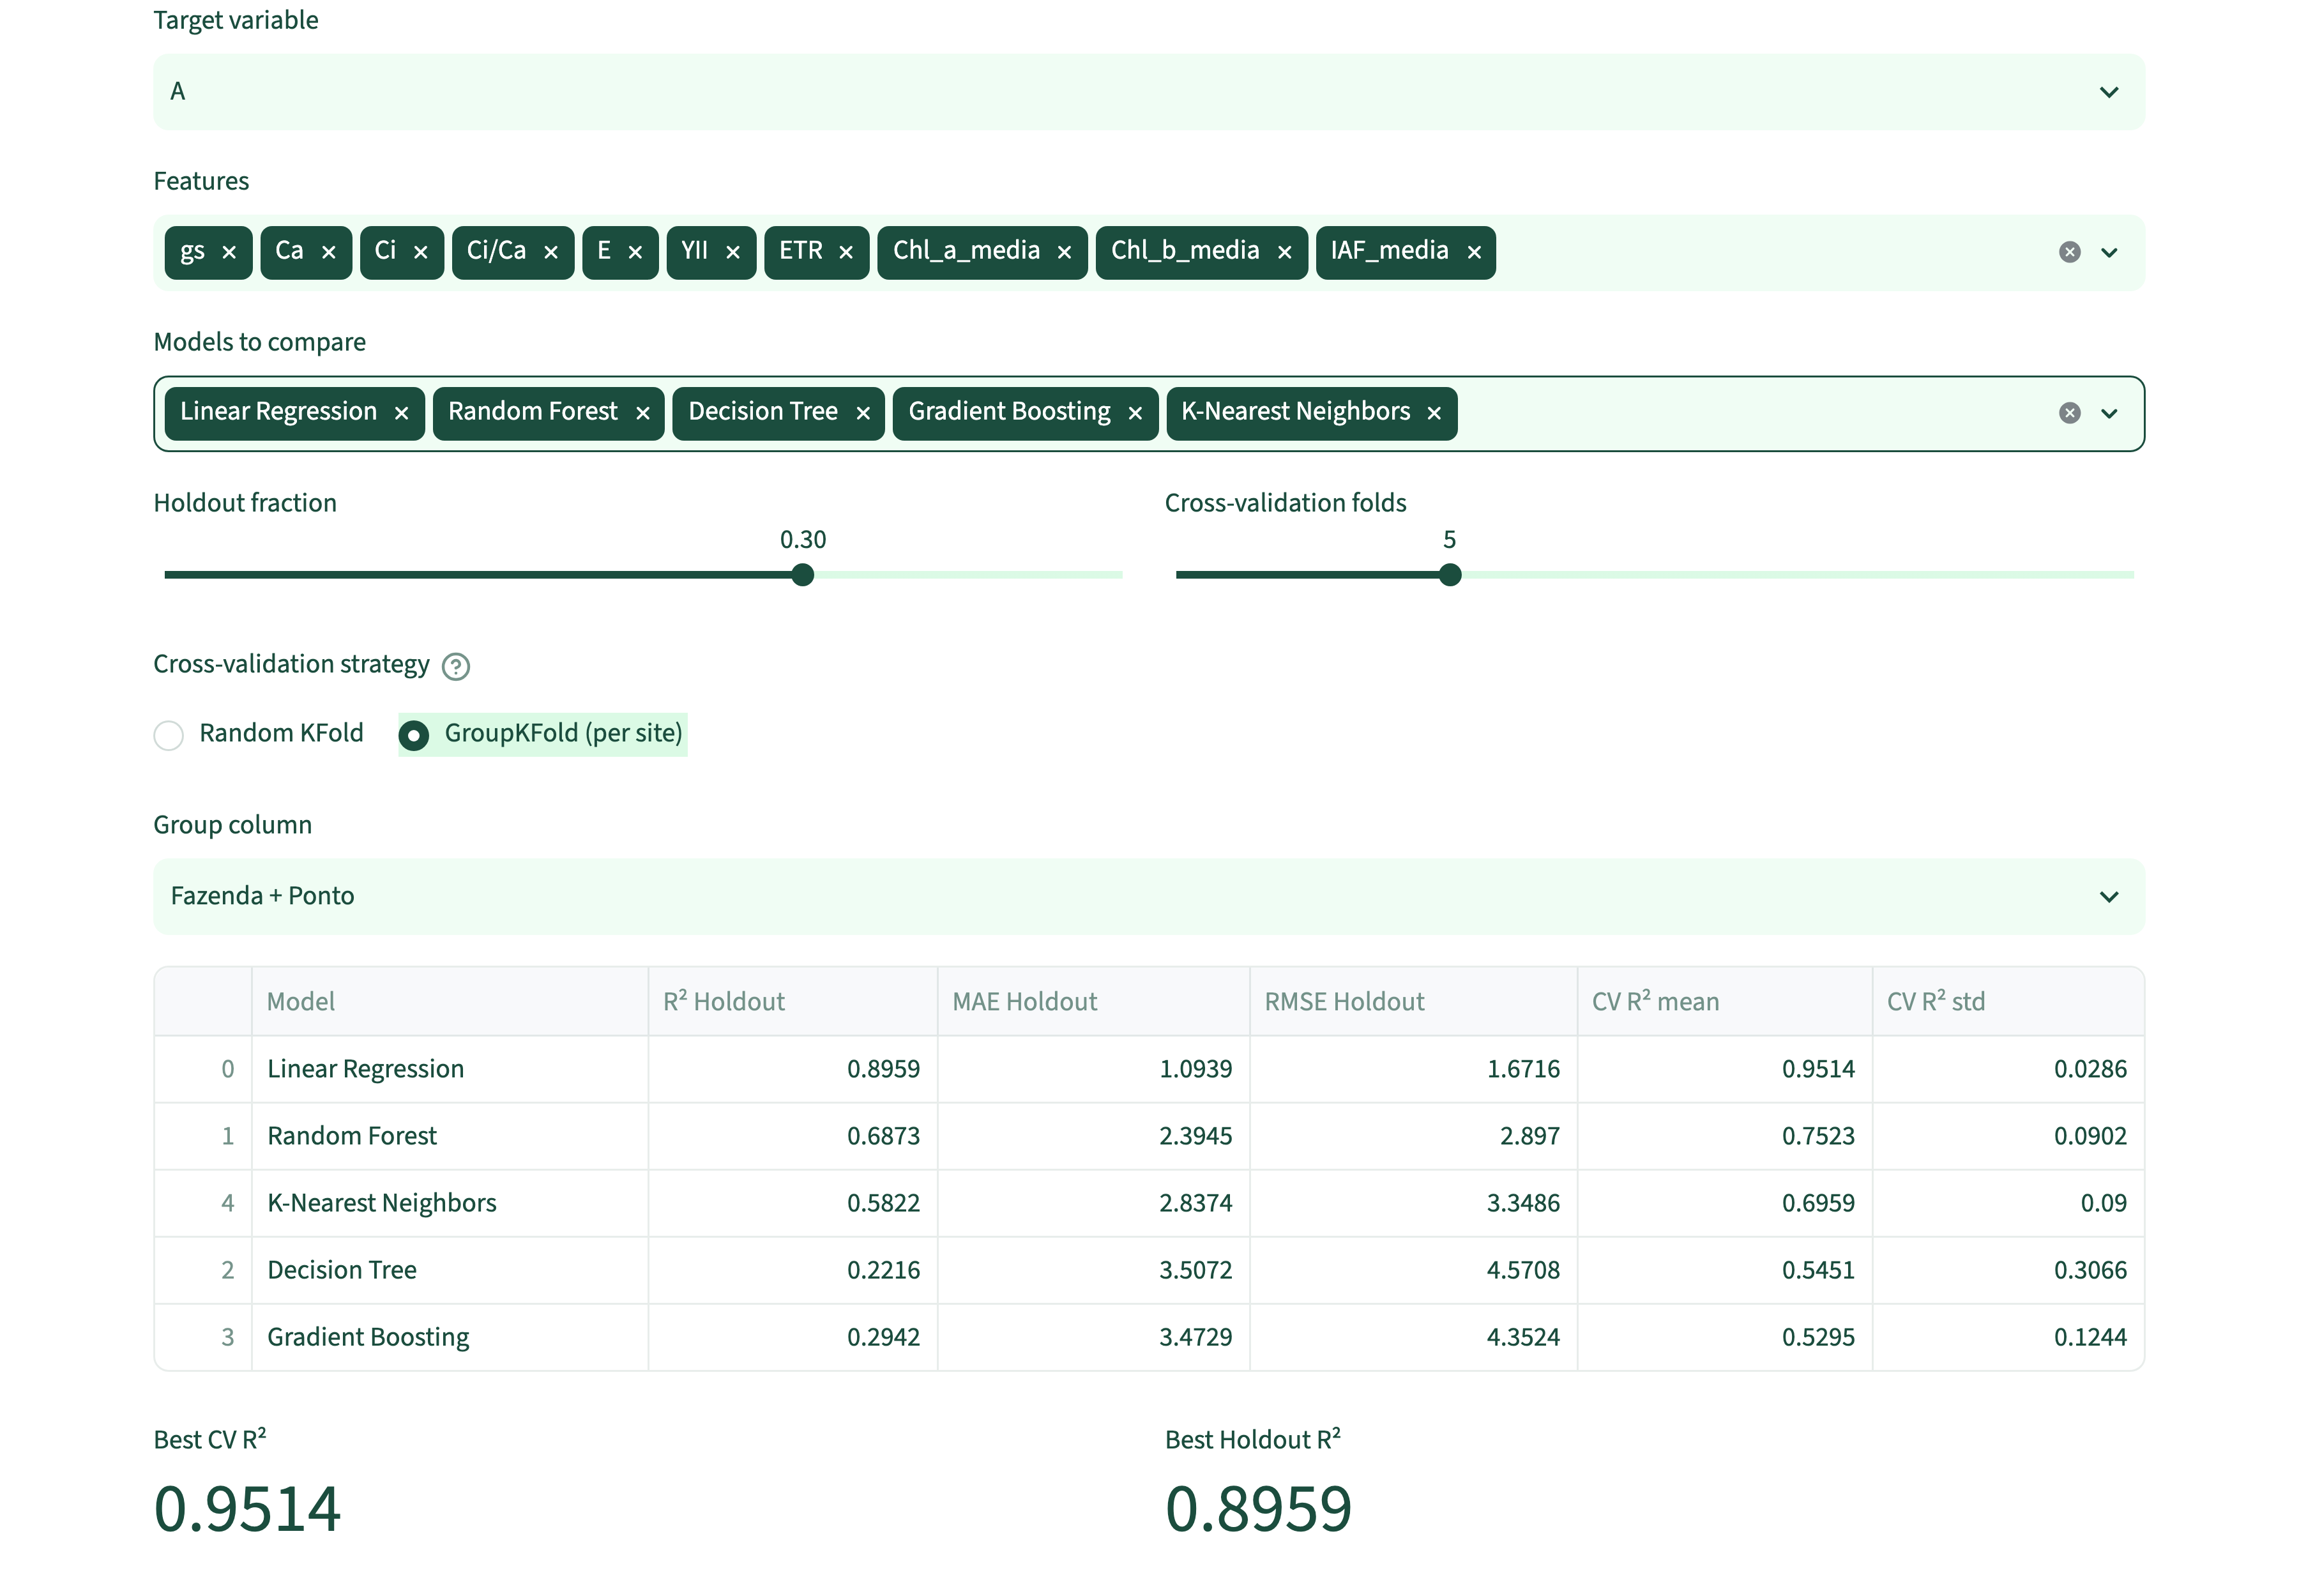
\includegraphics[width=\linewidth]{figs/modeling_comparison.png}
  \caption{Modelling page comparing five supervised regressors for net photosynthesis ($A$) on the Rio Verde dataset in a single run, reporting holdout $R^2$, MAE and RMSE alongside cross-validated $R^2$ (mean and standard deviation). Linear Regression attains the highest cross-validated skill, with the tree ensembles close behind; here the GroupKFold-per-site guard-rail (grouping on \emph{farm + point}) is enabled to curb pseudoreplication.}\label{fig:modeling}
\end{figure}

\begin{figure}[htbp]
  \centering
  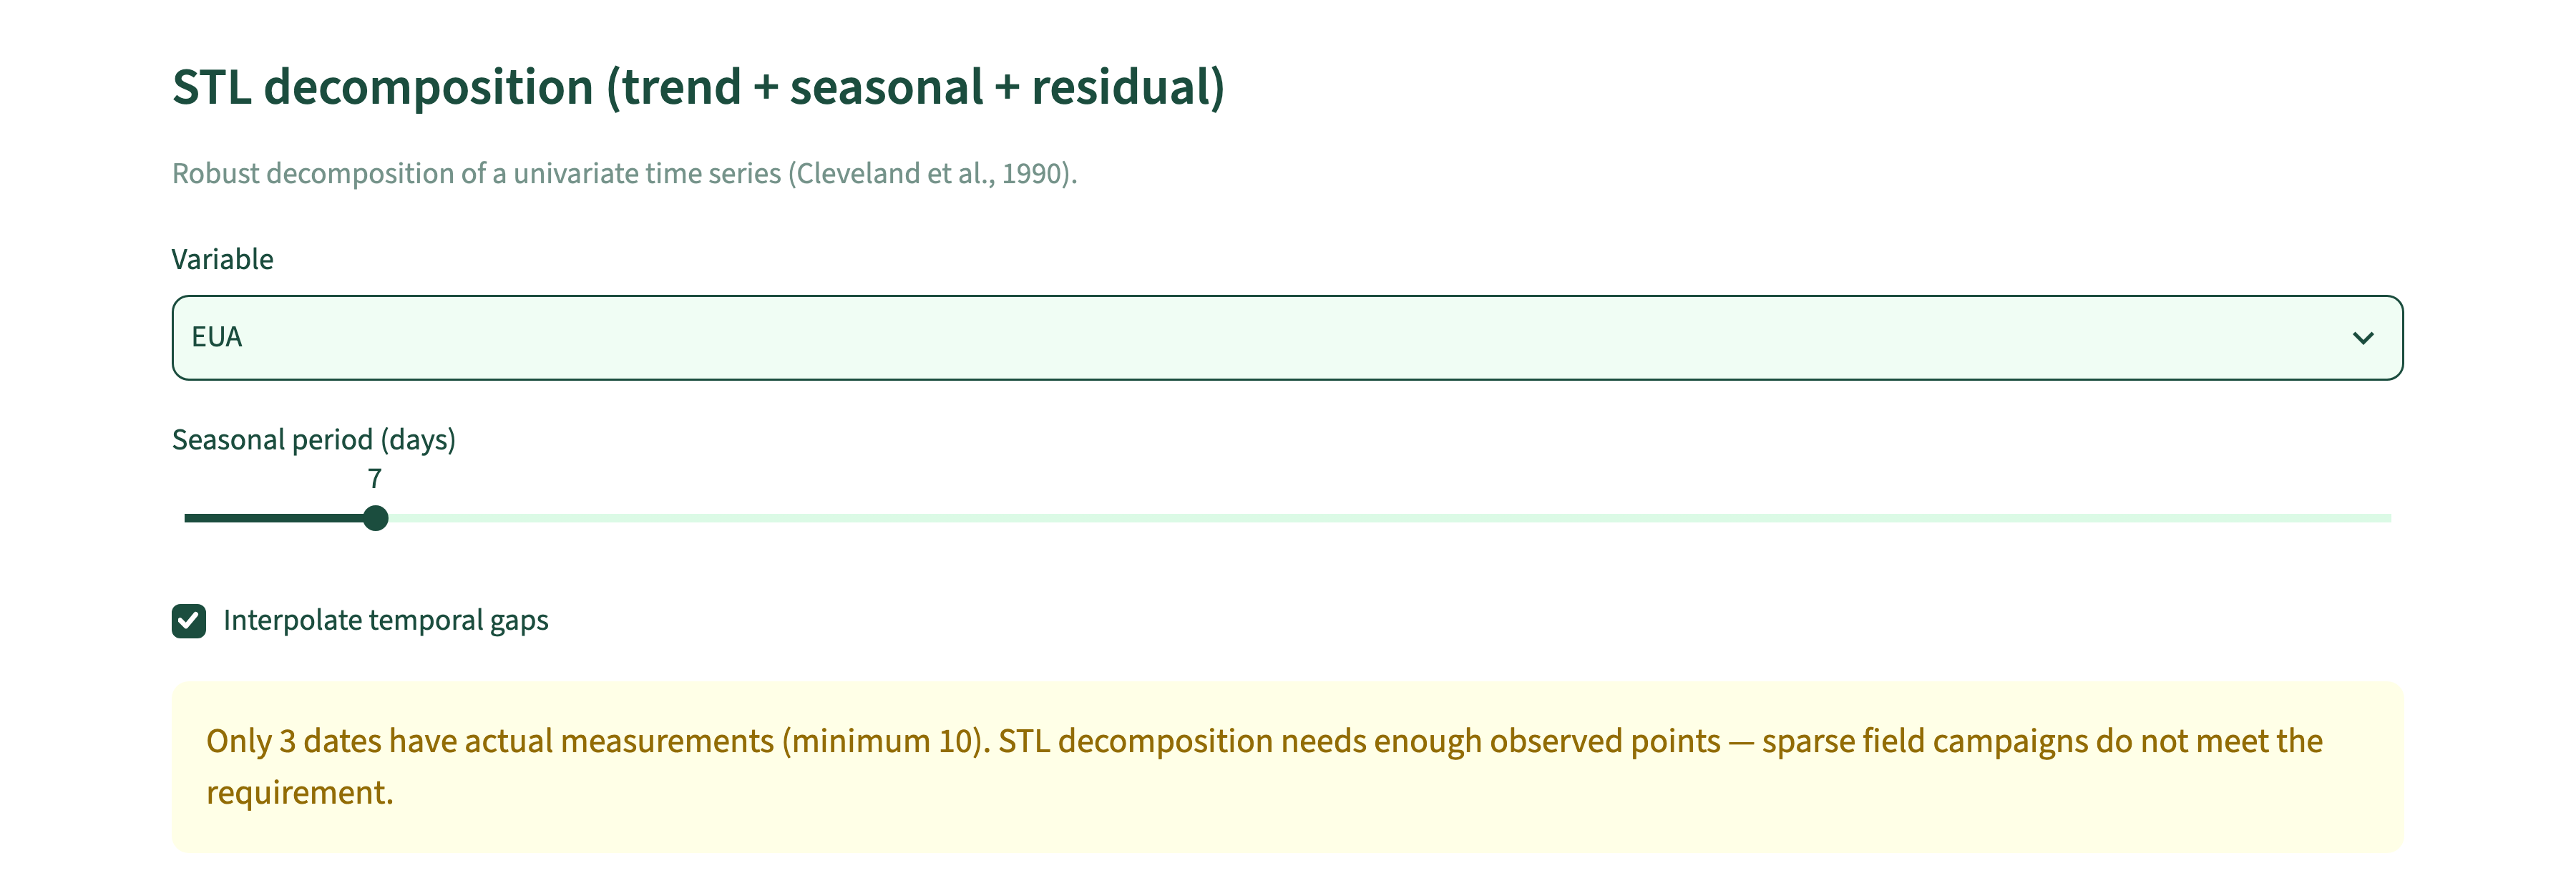
\includegraphics[width=\linewidth]{figs/stl_blocked.png}
  \caption{Time Series page on the Rio Verde dataset. Because the campaign contains only three distinct collection dates, below the ten-date threshold, the STL guard-rail blocks the decomposition and reports the reason instead of producing an interpolation-dominated result.}\label{fig:stl}
\end{figure}

\subsection{Datasets beyond ecophysiology}\label{sec:ex-generic}

To show that the platform is not bound to its original domain, we ran two public datasets through the same interface; in both, the profile resolver switched to the generic profile, so neither analysis required any change to the application.

The first is the classical Yates oats trial~\cite{Yates1935}, three oat varieties under four nitrogen rates across six blocks (72 rows), uploaded as a plain CSV and analysed on the Experimental-design page as a split-plot, with variety as the whole-plot factor and nitrogen as the sub-plot factor. The resulting ANOVA reproduces the reference fit from \texttt{nlme::Oats}~\cite{Pinheiro2000} to the decimal in every stratum (Table~\ref{tbl:oats}): the whole-plot variety effect is non-significant, the sub-plot nitrogen effect is strong, and the variety$\times$nitrogen interaction is negligible. The post-hoc Tukey test on nitrogen recovers the textbook dose response, yield saturating between the two highest rates, and the page's residual checks (Shapiro--Wilk, Levene) raise no flag.

\begin{table}[htbp]
\centering
\footnotesize
\begin{tabular}{lccc}
\toprule
\textbf{Term (stratum)} & \textbf{df} & \textbf{PhysioFlow $F$ ($p$)} & \textbf{\texttt{nlme::Oats} $F$ ($p$)} \\
\midrule
Variety (whole-plot)      & 2, 10 & 1.485 ($0.272$)        & 1.485 ($0.272$) \\
Nitrogen (sub-plot)       & 3, 45 & 37.686 ($<10^{-11}$)   & 37.686 ($<0.001$) \\
Variety $\times$ Nitrogen & 6, 45 & 0.303 ($0.932$)        & 0.303 ($0.932$) \\
\bottomrule
\end{tabular}
\caption{Split-plot ANOVA of the Yates oats trial computed by PhysioFlow's experimental-design module against the R \texttt{nlme::Oats} reference. The $F$ statistics match to the decimal in all three strata.}\label{tbl:oats}
\end{table}

The second is the Palmer penguins survey~\cite{Gorman2014}, a biology dataset of 344 morphometric records from three species. The EDA recovered the known flipper-length/body-mass correlation ($r=0.87$) and the sign reversal of bill depth against mass, a textbook instance of Simpson's paradox; in classification mode, Random Forest, SVM and $k$-NN separated the three species at $1.00$ holdout accuracy and $0.99$ under stratified cross-validation, matching the strongest published benchmarks. A split-plot agronomy trial and a biology survey thus run through the same guard-railed interface that served the gas-exchange campaign.

%% ====================================================================
\section{Impact overview}\label{sec:impact}

PhysioFlow brings the cleaning, exploratory analysis, supervised modelling and experimental-design analysis needed to interpret crop-ecophysiology data into a single platform. For researchers without a programming background, especially in under-resourced institutions, that barrier often delays the analysis of campaigns already expensive to run.

PhysioFlow's main contribution is methodological, not just operational: its statistical guard-rails turn assumptions that researchers usually check informally, or skip, into explicit on-screen warnings, steering non-statistician users away from confounding, multicollinearity, pseudoreplication and sparsity. In the Rio Verde campaign they caught a perfectly confounded design and a series too short for seasonal decomposition at once, problems that, left unflagged, would more likely have surfaced only at peer review.

\emph{PhysioFlow} is in routine use by two communities. Researchers of the Goi\'as Verde initiative (Instituto Federal Goiano and CEAGRE) apply it to soybean and sugarcane photosynthetic performance across Cerrado cropping systems, and graduate students of the Postgraduate Programme in Agricultural Sciences at Instituto Federal Goiano, Campus Rio Verde, use it to analyse their own experiments and as a teaching tool in data-analysis training. Because these users span plant physiology, agronomy and soil science, the same guard-railed interface serves both the research and the training pipeline of the group. The current release (v1.0) comprises about 7{,}400 lines of Python, 104 \texttt{pytest} tests and 771 user-interface keys, and early feedback from these users reports analyses that once took days of spreadsheet work now finishing in hours.

%% ====================================================================
\section{Limitations and future development}\label{sec:future}

PhysioFlow has known limitations. It targets tabular exports and does not read proprietary binary formats, so vendor files must first be exported to CSV, TSV or XLSX. The physiology profile recognises a fixed 31-column reference schema; datasets outside it fall back to the generic profile, where domain presets and instrument-specific replicate handling are unavailable. The experimental-design module assumes balanced or nearly balanced layouts, and it reports, but does not automatically correct, violated assumptions; severely unbalanced or missing-cell designs still require a dedicated mixed-model package. Finally, the application is session-based and holds the working dataset in memory, which bounds the size of campaigns it can process interactively on a standard laptop.

To date the platform has supported the analyses of the Goi\'as Verde initiative and the soil greenhouse-gas study presented at the 1st International Symposium on Climate and Agricultural Resilience~\cite{DaSilva2026Goias}; further studies on soybean and sugarcane photosynthetic performance in the Cerrado are in preparation, and this list will grow as ongoing campaigns are published.

Planned developments include physiological range validation in the schema (\texttt{valid\_range} per column), integration of the instrument data dictionary as in-app tooltips, raising test coverage above 70\% across the \texttt{ml/}, \texttt{state} and \texttt{auth} modules, a quasi-constant-variable warning in the correlation panel, and a public Docker image for one-command deployment. On the analytical side, automatic fitting of physiological response curves (e.g.\ $A$/$C_i$ and light-response curves), automated report export, and predictive guard-rails that flag physiological-stress patterns to support decision-making are planned as future directions.

%% ====================================================================
\section*{CRediT authorship contribution statement}
\textbf{Daniel Hil\'ario da Silva:} Conceptualization, Methodology, Software, Validation, Formal analysis, Investigation, Data curation, Visualization, Writing -- original draft, Writing -- review \& editing. \textbf{Leandro Rodrigues da Silva Souza:} Conceptualization, Methodology, Software, Supervision, Project administration, Funding acquisition, Writing -- review \& editing. \textbf{Andr\'e Abade:} Conceptualization, Methodology, Software, Validation, Writing -- review \& editing. \textbf{Francisco de Almeida Lobo:} Validation, Supervision, Writing -- review \& editing. \textbf{Fernando Rodrigues Cabral Filho:} Investigation, Data curation, Writing -- review \& editing. \textbf{Erli Pinto dos Santos:} Software, Visualization, Writing -- review \& editing. \textbf{Adinan Alves da Silva:} Investigation, Data curation, Resources. \textbf{Daiane Alves da Silva:} Investigation, Resources, Writing -- review \& editing. \textbf{Ketlyn Santos Sousa:} Investigation, Data curation, Writing -- review \& editing. \textbf{Igor Eli da Silva:} Software, Validation, Visualization. \textbf{Alan Carlos da Costa:} Supervision, Funding acquisition, Resources, Writing -- review \& editing.

%% ====================================================================
\section*{Declaration of competing interest}
The authors declare that they have no known competing financial interests or personal relationships that could have appeared to influence the work reported in this paper.

\section*{Data availability}
The source code, the documentation and the public datasets used in Section~\ref{sec:ex-generic} (Yates oats and Palmer penguins) are openly available in the repository listed in the Code metadata table, together with a synthetic ecophysiology dataset that reproduces the reference schema so that the full workflow can be re-run. The field campaign of Section~\ref{sec:ex-physio} belongs to an ongoing research project and cannot be released; the figures derived from it are de-identified.

%% ====================================================================
\section*{Acknowledgements}

The authors thank the Ministry of Science, Technology and Innovation (MCTI), the Brazilian Funding Authority for Studies and Projects (FINEP), the Goi\'as State Research Foundation (FAPEG), the National Council for Scientific and Technological Development (CNPq), the Coordination for the Improvement of Higher Education Personnel (CAPES), the State Secretariat for Development and Innovation of Goi\'as (SECTI), the Center of Excellence in Exponential Agriculture (CEAGRE), and the Instituto Federal Goiano for supporting the research developed.

%% ====================================================================
\bibliographystyle{unsrtnat}
\bibliography{refs}

\end{document}
